\begin{titlepage}
\thispagestyle{empty}
\begin{tikzpicture}[remember picture,overlay]
  \fill[white] (current page.south west) rectangle (current page.north east);
  \fill[Navy] (current page.north west) rectangle ([yshift=-8.25cm]current page.north east);
  \fill[Teal] ([yshift=-8.25cm]current page.north west) rectangle ([yshift=-8.60cm]current page.north east);
  \fill[Orange] ([yshift=-8.60cm]current page.north west) rectangle ([yshift=-8.73cm]current page.north east);
\end{tikzpicture}
\vspace*{1.7cm}
{\color{white}\sffamily\small FREE ENERGY TO LLMS\par}
\vspace{1.1cm}
{\color{white}\sffamily\fontsize{31}{38}\selectfont\bfseries 生成模型与概率统计\par}
\vspace{1.35cm}
{\centering\color{Navy}\sffamily\fontsize{16}{22}\selectfont 从变分自由能到大模型的推理和训练\par}
\vspace{2.5cm}
\begin{center}
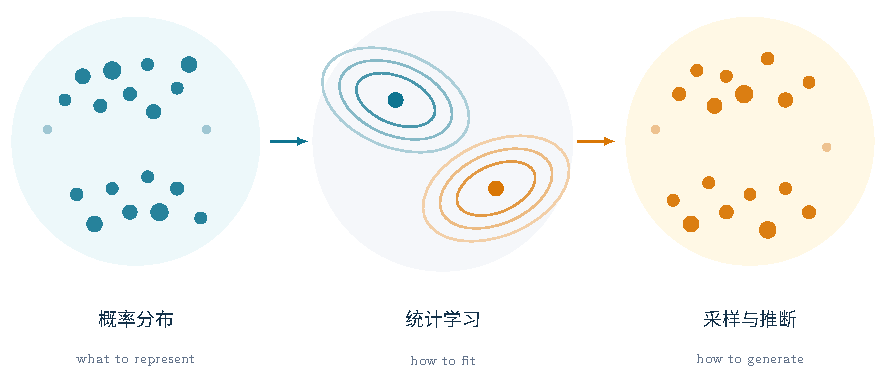
\includegraphics[width=0.96\textwidth]{cover_probability_flow.pdf}
\end{center}
\vfill
\begin{center}
\color{Navy}\sffamily\large 张士欣\par
\vspace{3mm}
\color{Slate}\normalsize 中国科学院物理研究所\quad 2026.10\par
\end{center}
\end{titlepage}
